
% Default to the notebook output style

    


% Inherit from the specified cell style.




    
\documentclass[11pt]{article}

    
    
    \usepackage[T1]{fontenc}
    % Nicer default font (+ math font) than Computer Modern for most use cases
    \usepackage{mathpazo}

    % Basic figure setup, for now with no caption control since it's done
    % automatically by Pandoc (which extracts ![](path) syntax from Markdown).
    \usepackage{graphicx}
    % We will generate all images so they have a width \maxwidth. This means
    % that they will get their normal width if they fit onto the page, but
    % are scaled down if they would overflow the margins.
    \makeatletter
    \def\maxwidth{\ifdim\Gin@nat@width>\linewidth\linewidth
    \else\Gin@nat@width\fi}
    \makeatother
    \let\Oldincludegraphics\includegraphics
    % Set max figure width to be 80% of text width, for now hardcoded.
    \renewcommand{\includegraphics}[1]{\Oldincludegraphics[width=.8\maxwidth]{#1}}
    % Ensure that by default, figures have no caption (until we provide a
    % proper Figure object with a Caption API and a way to capture that
    % in the conversion process - todo).
    \usepackage{caption}
    \DeclareCaptionLabelFormat{nolabel}{}
    \captionsetup{labelformat=nolabel}

    \usepackage{adjustbox} % Used to constrain images to a maximum size 
    \usepackage{xcolor} % Allow colors to be defined
    \usepackage{enumerate} % Needed for markdown enumerations to work
    \usepackage{geometry} % Used to adjust the document margins
    \usepackage{amsmath} % Equations
    \usepackage{amssymb} % Equations
    \usepackage{textcomp} % defines textquotesingle
    % Hack from http://tex.stackexchange.com/a/47451/13684:
    \AtBeginDocument{%
        \def\PYZsq{\textquotesingle}% Upright quotes in Pygmentized code
    }
    \usepackage{upquote} % Upright quotes for verbatim code
    \usepackage{eurosym} % defines \euro
    \usepackage[mathletters]{ucs} % Extended unicode (utf-8) support
    \usepackage[utf8x]{inputenc} % Allow utf-8 characters in the tex document
    \usepackage{fancyvrb} % verbatim replacement that allows latex
    \usepackage{grffile} % extends the file name processing of package graphics 
                         % to support a larger range 
    % The hyperref package gives us a pdf with properly built
    % internal navigation ('pdf bookmarks' for the table of contents,
    % internal cross-reference links, web links for URLs, etc.)
    \usepackage{hyperref}
    \usepackage{longtable} % longtable support required by pandoc >1.10
    \usepackage{booktabs}  % table support for pandoc > 1.12.2
    \usepackage[inline]{enumitem} % IRkernel/repr support (it uses the enumerate* environment)
    \usepackage[normalem]{ulem} % ulem is needed to support strikethroughs (\sout)
                                % normalem makes italics be italics, not underlines
    

    
    
    % Colors for the hyperref package
    \definecolor{urlcolor}{rgb}{0,.145,.698}
    \definecolor{linkcolor}{rgb}{.71,0.21,0.01}
    \definecolor{citecolor}{rgb}{.12,.54,.11}

    % ANSI colors
    \definecolor{ansi-black}{HTML}{3E424D}
    \definecolor{ansi-black-intense}{HTML}{282C36}
    \definecolor{ansi-red}{HTML}{E75C58}
    \definecolor{ansi-red-intense}{HTML}{B22B31}
    \definecolor{ansi-green}{HTML}{00A250}
    \definecolor{ansi-green-intense}{HTML}{007427}
    \definecolor{ansi-yellow}{HTML}{DDB62B}
    \definecolor{ansi-yellow-intense}{HTML}{B27D12}
    \definecolor{ansi-blue}{HTML}{208FFB}
    \definecolor{ansi-blue-intense}{HTML}{0065CA}
    \definecolor{ansi-magenta}{HTML}{D160C4}
    \definecolor{ansi-magenta-intense}{HTML}{A03196}
    \definecolor{ansi-cyan}{HTML}{60C6C8}
    \definecolor{ansi-cyan-intense}{HTML}{258F8F}
    \definecolor{ansi-white}{HTML}{C5C1B4}
    \definecolor{ansi-white-intense}{HTML}{A1A6B2}

    % commands and environments needed by pandoc snippets
    % extracted from the output of `pandoc -s`
    \providecommand{\tightlist}{%
      \setlength{\itemsep}{0pt}\setlength{\parskip}{0pt}}
    \DefineVerbatimEnvironment{Highlighting}{Verbatim}{commandchars=\\\{\}}
    % Add ',fontsize=\small' for more characters per line
    \newenvironment{Shaded}{}{}
    \newcommand{\KeywordTok}[1]{\textcolor[rgb]{0.00,0.44,0.13}{\textbf{{#1}}}}
    \newcommand{\DataTypeTok}[1]{\textcolor[rgb]{0.56,0.13,0.00}{{#1}}}
    \newcommand{\DecValTok}[1]{\textcolor[rgb]{0.25,0.63,0.44}{{#1}}}
    \newcommand{\BaseNTok}[1]{\textcolor[rgb]{0.25,0.63,0.44}{{#1}}}
    \newcommand{\FloatTok}[1]{\textcolor[rgb]{0.25,0.63,0.44}{{#1}}}
    \newcommand{\CharTok}[1]{\textcolor[rgb]{0.25,0.44,0.63}{{#1}}}
    \newcommand{\StringTok}[1]{\textcolor[rgb]{0.25,0.44,0.63}{{#1}}}
    \newcommand{\CommentTok}[1]{\textcolor[rgb]{0.38,0.63,0.69}{\textit{{#1}}}}
    \newcommand{\OtherTok}[1]{\textcolor[rgb]{0.00,0.44,0.13}{{#1}}}
    \newcommand{\AlertTok}[1]{\textcolor[rgb]{1.00,0.00,0.00}{\textbf{{#1}}}}
    \newcommand{\FunctionTok}[1]{\textcolor[rgb]{0.02,0.16,0.49}{{#1}}}
    \newcommand{\RegionMarkerTok}[1]{{#1}}
    \newcommand{\ErrorTok}[1]{\textcolor[rgb]{1.00,0.00,0.00}{\textbf{{#1}}}}
    \newcommand{\NormalTok}[1]{{#1}}
    
    % Additional commands for more recent versions of Pandoc
    \newcommand{\ConstantTok}[1]{\textcolor[rgb]{0.53,0.00,0.00}{{#1}}}
    \newcommand{\SpecialCharTok}[1]{\textcolor[rgb]{0.25,0.44,0.63}{{#1}}}
    \newcommand{\VerbatimStringTok}[1]{\textcolor[rgb]{0.25,0.44,0.63}{{#1}}}
    \newcommand{\SpecialStringTok}[1]{\textcolor[rgb]{0.73,0.40,0.53}{{#1}}}
    \newcommand{\ImportTok}[1]{{#1}}
    \newcommand{\DocumentationTok}[1]{\textcolor[rgb]{0.73,0.13,0.13}{\textit{{#1}}}}
    \newcommand{\AnnotationTok}[1]{\textcolor[rgb]{0.38,0.63,0.69}{\textbf{\textit{{#1}}}}}
    \newcommand{\CommentVarTok}[1]{\textcolor[rgb]{0.38,0.63,0.69}{\textbf{\textit{{#1}}}}}
    \newcommand{\VariableTok}[1]{\textcolor[rgb]{0.10,0.09,0.49}{{#1}}}
    \newcommand{\ControlFlowTok}[1]{\textcolor[rgb]{0.00,0.44,0.13}{\textbf{{#1}}}}
    \newcommand{\OperatorTok}[1]{\textcolor[rgb]{0.40,0.40,0.40}{{#1}}}
    \newcommand{\BuiltInTok}[1]{{#1}}
    \newcommand{\ExtensionTok}[1]{{#1}}
    \newcommand{\PreprocessorTok}[1]{\textcolor[rgb]{0.74,0.48,0.00}{{#1}}}
    \newcommand{\AttributeTok}[1]{\textcolor[rgb]{0.49,0.56,0.16}{{#1}}}
    \newcommand{\InformationTok}[1]{\textcolor[rgb]{0.38,0.63,0.69}{\textbf{\textit{{#1}}}}}
    \newcommand{\WarningTok}[1]{\textcolor[rgb]{0.38,0.63,0.69}{\textbf{\textit{{#1}}}}}
    
    
    % Define a nice break command that doesn't care if a line doesn't already
    % exist.
    \def\br{\hspace*{\fill} \\* }
    % Math Jax compatability definitions
    \def\gt{>}
    \def\lt{<}
    % Document parameters
    \title{Project}
    
    
    

    % Pygments definitions
    
\makeatletter
\def\PY@reset{\let\PY@it=\relax \let\PY@bf=\relax%
    \let\PY@ul=\relax \let\PY@tc=\relax%
    \let\PY@bc=\relax \let\PY@ff=\relax}
\def\PY@tok#1{\csname PY@tok@#1\endcsname}
\def\PY@toks#1+{\ifx\relax#1\empty\else%
    \PY@tok{#1}\expandafter\PY@toks\fi}
\def\PY@do#1{\PY@bc{\PY@tc{\PY@ul{%
    \PY@it{\PY@bf{\PY@ff{#1}}}}}}}
\def\PY#1#2{\PY@reset\PY@toks#1+\relax+\PY@do{#2}}

\expandafter\def\csname PY@tok@gd\endcsname{\def\PY@tc##1{\textcolor[rgb]{0.63,0.00,0.00}{##1}}}
\expandafter\def\csname PY@tok@gu\endcsname{\let\PY@bf=\textbf\def\PY@tc##1{\textcolor[rgb]{0.50,0.00,0.50}{##1}}}
\expandafter\def\csname PY@tok@gt\endcsname{\def\PY@tc##1{\textcolor[rgb]{0.00,0.27,0.87}{##1}}}
\expandafter\def\csname PY@tok@gs\endcsname{\let\PY@bf=\textbf}
\expandafter\def\csname PY@tok@gr\endcsname{\def\PY@tc##1{\textcolor[rgb]{1.00,0.00,0.00}{##1}}}
\expandafter\def\csname PY@tok@cm\endcsname{\let\PY@it=\textit\def\PY@tc##1{\textcolor[rgb]{0.25,0.50,0.50}{##1}}}
\expandafter\def\csname PY@tok@vg\endcsname{\def\PY@tc##1{\textcolor[rgb]{0.10,0.09,0.49}{##1}}}
\expandafter\def\csname PY@tok@vi\endcsname{\def\PY@tc##1{\textcolor[rgb]{0.10,0.09,0.49}{##1}}}
\expandafter\def\csname PY@tok@vm\endcsname{\def\PY@tc##1{\textcolor[rgb]{0.10,0.09,0.49}{##1}}}
\expandafter\def\csname PY@tok@mh\endcsname{\def\PY@tc##1{\textcolor[rgb]{0.40,0.40,0.40}{##1}}}
\expandafter\def\csname PY@tok@cs\endcsname{\let\PY@it=\textit\def\PY@tc##1{\textcolor[rgb]{0.25,0.50,0.50}{##1}}}
\expandafter\def\csname PY@tok@ge\endcsname{\let\PY@it=\textit}
\expandafter\def\csname PY@tok@vc\endcsname{\def\PY@tc##1{\textcolor[rgb]{0.10,0.09,0.49}{##1}}}
\expandafter\def\csname PY@tok@il\endcsname{\def\PY@tc##1{\textcolor[rgb]{0.40,0.40,0.40}{##1}}}
\expandafter\def\csname PY@tok@go\endcsname{\def\PY@tc##1{\textcolor[rgb]{0.53,0.53,0.53}{##1}}}
\expandafter\def\csname PY@tok@cp\endcsname{\def\PY@tc##1{\textcolor[rgb]{0.74,0.48,0.00}{##1}}}
\expandafter\def\csname PY@tok@gi\endcsname{\def\PY@tc##1{\textcolor[rgb]{0.00,0.63,0.00}{##1}}}
\expandafter\def\csname PY@tok@gh\endcsname{\let\PY@bf=\textbf\def\PY@tc##1{\textcolor[rgb]{0.00,0.00,0.50}{##1}}}
\expandafter\def\csname PY@tok@ni\endcsname{\let\PY@bf=\textbf\def\PY@tc##1{\textcolor[rgb]{0.60,0.60,0.60}{##1}}}
\expandafter\def\csname PY@tok@nl\endcsname{\def\PY@tc##1{\textcolor[rgb]{0.63,0.63,0.00}{##1}}}
\expandafter\def\csname PY@tok@nn\endcsname{\let\PY@bf=\textbf\def\PY@tc##1{\textcolor[rgb]{0.00,0.00,1.00}{##1}}}
\expandafter\def\csname PY@tok@no\endcsname{\def\PY@tc##1{\textcolor[rgb]{0.53,0.00,0.00}{##1}}}
\expandafter\def\csname PY@tok@na\endcsname{\def\PY@tc##1{\textcolor[rgb]{0.49,0.56,0.16}{##1}}}
\expandafter\def\csname PY@tok@nb\endcsname{\def\PY@tc##1{\textcolor[rgb]{0.00,0.50,0.00}{##1}}}
\expandafter\def\csname PY@tok@nc\endcsname{\let\PY@bf=\textbf\def\PY@tc##1{\textcolor[rgb]{0.00,0.00,1.00}{##1}}}
\expandafter\def\csname PY@tok@nd\endcsname{\def\PY@tc##1{\textcolor[rgb]{0.67,0.13,1.00}{##1}}}
\expandafter\def\csname PY@tok@ne\endcsname{\let\PY@bf=\textbf\def\PY@tc##1{\textcolor[rgb]{0.82,0.25,0.23}{##1}}}
\expandafter\def\csname PY@tok@nf\endcsname{\def\PY@tc##1{\textcolor[rgb]{0.00,0.00,1.00}{##1}}}
\expandafter\def\csname PY@tok@si\endcsname{\let\PY@bf=\textbf\def\PY@tc##1{\textcolor[rgb]{0.73,0.40,0.53}{##1}}}
\expandafter\def\csname PY@tok@s2\endcsname{\def\PY@tc##1{\textcolor[rgb]{0.73,0.13,0.13}{##1}}}
\expandafter\def\csname PY@tok@nt\endcsname{\let\PY@bf=\textbf\def\PY@tc##1{\textcolor[rgb]{0.00,0.50,0.00}{##1}}}
\expandafter\def\csname PY@tok@nv\endcsname{\def\PY@tc##1{\textcolor[rgb]{0.10,0.09,0.49}{##1}}}
\expandafter\def\csname PY@tok@s1\endcsname{\def\PY@tc##1{\textcolor[rgb]{0.73,0.13,0.13}{##1}}}
\expandafter\def\csname PY@tok@dl\endcsname{\def\PY@tc##1{\textcolor[rgb]{0.73,0.13,0.13}{##1}}}
\expandafter\def\csname PY@tok@ch\endcsname{\let\PY@it=\textit\def\PY@tc##1{\textcolor[rgb]{0.25,0.50,0.50}{##1}}}
\expandafter\def\csname PY@tok@m\endcsname{\def\PY@tc##1{\textcolor[rgb]{0.40,0.40,0.40}{##1}}}
\expandafter\def\csname PY@tok@gp\endcsname{\let\PY@bf=\textbf\def\PY@tc##1{\textcolor[rgb]{0.00,0.00,0.50}{##1}}}
\expandafter\def\csname PY@tok@sh\endcsname{\def\PY@tc##1{\textcolor[rgb]{0.73,0.13,0.13}{##1}}}
\expandafter\def\csname PY@tok@ow\endcsname{\let\PY@bf=\textbf\def\PY@tc##1{\textcolor[rgb]{0.67,0.13,1.00}{##1}}}
\expandafter\def\csname PY@tok@sx\endcsname{\def\PY@tc##1{\textcolor[rgb]{0.00,0.50,0.00}{##1}}}
\expandafter\def\csname PY@tok@bp\endcsname{\def\PY@tc##1{\textcolor[rgb]{0.00,0.50,0.00}{##1}}}
\expandafter\def\csname PY@tok@c1\endcsname{\let\PY@it=\textit\def\PY@tc##1{\textcolor[rgb]{0.25,0.50,0.50}{##1}}}
\expandafter\def\csname PY@tok@fm\endcsname{\def\PY@tc##1{\textcolor[rgb]{0.00,0.00,1.00}{##1}}}
\expandafter\def\csname PY@tok@o\endcsname{\def\PY@tc##1{\textcolor[rgb]{0.40,0.40,0.40}{##1}}}
\expandafter\def\csname PY@tok@kc\endcsname{\let\PY@bf=\textbf\def\PY@tc##1{\textcolor[rgb]{0.00,0.50,0.00}{##1}}}
\expandafter\def\csname PY@tok@c\endcsname{\let\PY@it=\textit\def\PY@tc##1{\textcolor[rgb]{0.25,0.50,0.50}{##1}}}
\expandafter\def\csname PY@tok@mf\endcsname{\def\PY@tc##1{\textcolor[rgb]{0.40,0.40,0.40}{##1}}}
\expandafter\def\csname PY@tok@err\endcsname{\def\PY@bc##1{\setlength{\fboxsep}{0pt}\fcolorbox[rgb]{1.00,0.00,0.00}{1,1,1}{\strut ##1}}}
\expandafter\def\csname PY@tok@mb\endcsname{\def\PY@tc##1{\textcolor[rgb]{0.40,0.40,0.40}{##1}}}
\expandafter\def\csname PY@tok@ss\endcsname{\def\PY@tc##1{\textcolor[rgb]{0.10,0.09,0.49}{##1}}}
\expandafter\def\csname PY@tok@sr\endcsname{\def\PY@tc##1{\textcolor[rgb]{0.73,0.40,0.53}{##1}}}
\expandafter\def\csname PY@tok@mo\endcsname{\def\PY@tc##1{\textcolor[rgb]{0.40,0.40,0.40}{##1}}}
\expandafter\def\csname PY@tok@kd\endcsname{\let\PY@bf=\textbf\def\PY@tc##1{\textcolor[rgb]{0.00,0.50,0.00}{##1}}}
\expandafter\def\csname PY@tok@mi\endcsname{\def\PY@tc##1{\textcolor[rgb]{0.40,0.40,0.40}{##1}}}
\expandafter\def\csname PY@tok@kn\endcsname{\let\PY@bf=\textbf\def\PY@tc##1{\textcolor[rgb]{0.00,0.50,0.00}{##1}}}
\expandafter\def\csname PY@tok@cpf\endcsname{\let\PY@it=\textit\def\PY@tc##1{\textcolor[rgb]{0.25,0.50,0.50}{##1}}}
\expandafter\def\csname PY@tok@kr\endcsname{\let\PY@bf=\textbf\def\PY@tc##1{\textcolor[rgb]{0.00,0.50,0.00}{##1}}}
\expandafter\def\csname PY@tok@s\endcsname{\def\PY@tc##1{\textcolor[rgb]{0.73,0.13,0.13}{##1}}}
\expandafter\def\csname PY@tok@kp\endcsname{\def\PY@tc##1{\textcolor[rgb]{0.00,0.50,0.00}{##1}}}
\expandafter\def\csname PY@tok@w\endcsname{\def\PY@tc##1{\textcolor[rgb]{0.73,0.73,0.73}{##1}}}
\expandafter\def\csname PY@tok@kt\endcsname{\def\PY@tc##1{\textcolor[rgb]{0.69,0.00,0.25}{##1}}}
\expandafter\def\csname PY@tok@sc\endcsname{\def\PY@tc##1{\textcolor[rgb]{0.73,0.13,0.13}{##1}}}
\expandafter\def\csname PY@tok@sb\endcsname{\def\PY@tc##1{\textcolor[rgb]{0.73,0.13,0.13}{##1}}}
\expandafter\def\csname PY@tok@sa\endcsname{\def\PY@tc##1{\textcolor[rgb]{0.73,0.13,0.13}{##1}}}
\expandafter\def\csname PY@tok@k\endcsname{\let\PY@bf=\textbf\def\PY@tc##1{\textcolor[rgb]{0.00,0.50,0.00}{##1}}}
\expandafter\def\csname PY@tok@se\endcsname{\let\PY@bf=\textbf\def\PY@tc##1{\textcolor[rgb]{0.73,0.40,0.13}{##1}}}
\expandafter\def\csname PY@tok@sd\endcsname{\let\PY@it=\textit\def\PY@tc##1{\textcolor[rgb]{0.73,0.13,0.13}{##1}}}

\def\PYZbs{\char`\\}
\def\PYZus{\char`\_}
\def\PYZob{\char`\{}
\def\PYZcb{\char`\}}
\def\PYZca{\char`\^}
\def\PYZam{\char`\&}
\def\PYZlt{\char`\<}
\def\PYZgt{\char`\>}
\def\PYZsh{\char`\#}
\def\PYZpc{\char`\%}
\def\PYZdl{\char`\$}
\def\PYZhy{\char`\-}
\def\PYZsq{\char`\'}
\def\PYZdq{\char`\"}
\def\PYZti{\char`\~}
% for compatibility with earlier versions
\def\PYZat{@}
\def\PYZlb{[}
\def\PYZrb{]}
\makeatother


    % Exact colors from NB
    \definecolor{incolor}{rgb}{0.0, 0.0, 0.5}
    \definecolor{outcolor}{rgb}{0.545, 0.0, 0.0}



    
    % Prevent overflowing lines due to hard-to-break entities
    \sloppy 
    % Setup hyperref package
    \hypersetup{
      breaklinks=true,  % so long urls are correctly broken across lines
      colorlinks=true,
      urlcolor=urlcolor,
      linkcolor=linkcolor,
      citecolor=citecolor,
      }
    % Slightly bigger margins than the latex defaults
    
    \geometry{verbose,tmargin=1in,bmargin=1in,lmargin=1in,rmargin=1in}
    
    

    \begin{document}
    
    
    \maketitle
    
    

    
    \begin{Verbatim}[commandchars=\\\{\}]
{\color{incolor}In [{\color{incolor}1}]:} \PY{k+kn}{import} \PY{n+nn}{numpy}
        \PY{k+kn}{import} \PY{n+nn}{pandas}
        
        \PY{k+kn}{from} \PY{n+nn}{sklearn.model\PYZus{}selection} \PY{k+kn}{import} \PY{n}{train\PYZus{}test\PYZus{}split}
        
        \PY{k+kn}{from} \PY{n+nn}{sklearn.metrics} \PY{k+kn}{import} \PY{n}{average\PYZus{}precision\PYZus{}score}
        \PY{k+kn}{from} \PY{n+nn}{sklearn.metrics} \PY{k+kn}{import} \PY{n}{precision\PYZus{}recall\PYZus{}curve}
        
        \PY{k+kn}{from} \PY{n+nn}{sklearn} \PY{k+kn}{import} \PY{n}{svm}
\end{Verbatim}


    \begin{Verbatim}[commandchars=\\\{\}]
{\color{incolor}In [{\color{incolor}2}]:} \PY{c+c1}{\PYZsh{}\PYZsh{} https://archive.ics.uci.edu/ml/machine\PYZhy{}learning\PYZhy{}databases/breast\PYZhy{}cancer\PYZhy{}wisconsin/breast\PYZhy{}cancer\PYZhy{}wisconsin.names}
        
        \PY{n}{HEADERS} \PY{o}{=} \PY{p}{[}\PY{l+s+s2}{\PYZdq{}}\PY{l+s+s2}{Sample code number}\PY{l+s+s2}{\PYZdq{}}\PY{p}{,}\PY{l+s+s2}{\PYZdq{}}\PY{l+s+s2}{Clump Thickness}\PY{l+s+s2}{\PYZdq{}}\PY{p}{,}\PY{l+s+s2}{\PYZdq{}}\PY{l+s+s2}{Uniformity of Cell Size}\PY{l+s+s2}{\PYZdq{}}\PY{p}{,}\PY{l+s+s2}{\PYZdq{}}\PY{l+s+s2}{Uniformity of Cell Shape}\PY{l+s+s2}{\PYZdq{}}\PY{p}{,}
                   \PY{l+s+s2}{\PYZdq{}}\PY{l+s+s2}{Marginal Adhesion}\PY{l+s+s2}{\PYZdq{}}\PY{p}{,}\PY{l+s+s2}{\PYZdq{}}\PY{l+s+s2}{Single Epithelial Cell Size}\PY{l+s+s2}{\PYZdq{}}\PY{p}{,}\PY{l+s+s2}{\PYZdq{}}\PY{l+s+s2}{Bare Nuclei}\PY{l+s+s2}{\PYZdq{}}\PY{p}{,}\PY{l+s+s2}{\PYZdq{}}\PY{l+s+s2}{Bland Chromatin}\PY{l+s+s2}{\PYZdq{}}\PY{p}{,}
                   \PY{l+s+s2}{\PYZdq{}}\PY{l+s+s2}{Normal Nucleoli}\PY{l+s+s2}{\PYZdq{}}\PY{p}{,}\PY{l+s+s2}{\PYZdq{}}\PY{l+s+s2}{Mitoses}\PY{l+s+s2}{\PYZdq{}}\PY{p}{,}\PY{l+s+s2}{\PYZdq{}}\PY{l+s+s2}{Class}\PY{l+s+s2}{\PYZdq{}}\PY{p}{]}
        
        \PY{n}{dataset} \PY{o}{=} \PY{n}{pandas}\PY{o}{.}\PY{n}{read\PYZus{}csv}\PY{p}{(}\PY{l+s+s2}{\PYZdq{}}\PY{l+s+s2}{breast\PYZhy{}cancer\PYZhy{}wisconsin.data}\PY{l+s+s2}{\PYZdq{}}\PY{p}{,} \PY{n}{names}\PY{o}{=}\PY{n}{HEADERS}\PY{p}{,} \PY{n}{low\PYZus{}memory}\PY{o}{=}\PY{n+nb+bp}{False}\PY{p}{)}
\end{Verbatim}


    \subsection{Import data}\label{import-data}

    \begin{Verbatim}[commandchars=\\\{\}]
{\color{incolor}In [{\color{incolor}3}]:} \PY{n}{dataset}\PY{o}{.}\PY{n}{dtypes}
\end{Verbatim}


\begin{Verbatim}[commandchars=\\\{\}]
{\color{outcolor}Out[{\color{outcolor}3}]:} Sample code number              int64
        Clump Thickness                 int64
        Uniformity of Cell Size         int64
        Uniformity of Cell Shape        int64
        Marginal Adhesion               int64
        Single Epithelial Cell Size     int64
        Bare Nuclei                    object
        Bland Chromatin                 int64
        Normal Nucleoli                 int64
        Mitoses                         int64
        Class                           int64
        dtype: object
\end{Verbatim}
            
    \begin{Verbatim}[commandchars=\\\{\}]
{\color{incolor}In [{\color{incolor}4}]:} \PY{n}{dataset}\PY{o}{.}\PY{n}{head}\PY{p}{(}\PY{p}{)}
\end{Verbatim}


\begin{Verbatim}[commandchars=\\\{\}]
{\color{outcolor}Out[{\color{outcolor}4}]:}    Sample code number  Clump Thickness  Uniformity of Cell Size  \textbackslash{}
        0             1000025                5                        1   
        1             1002945                5                        4   
        2             1015425                3                        1   
        3             1016277                6                        8   
        4             1017023                4                        1   
        
           Uniformity of Cell Shape  Marginal Adhesion  Single Epithelial Cell Size  \textbackslash{}
        0                         1                  1                            2   
        1                         4                  5                            7   
        2                         1                  1                            2   
        3                         8                  1                            3   
        4                         1                  3                            2   
        
          Bare Nuclei  Bland Chromatin  Normal Nucleoli  Mitoses  Class  
        0           1                3                1        1      2  
        1          10                3                2        1      2  
        2           2                3                1        1      2  
        3           4                3                7        1      2  
        4           1                3                1        1      2  
\end{Verbatim}
            
    \begin{Verbatim}[commandchars=\\\{\}]
{\color{incolor}In [{\color{incolor}5}]:} \PY{n}{dataset}\PY{o}{.}\PY{n}{shape}
\end{Verbatim}


\begin{Verbatim}[commandchars=\\\{\}]
{\color{outcolor}Out[{\color{outcolor}5}]:} (699, 11)
\end{Verbatim}
            
    \begin{Verbatim}[commandchars=\\\{\}]
{\color{incolor}In [{\color{incolor}6}]:} \PY{n}{dataset}\PY{o}{.}\PY{n}{describe}\PY{p}{(}\PY{p}{)}
\end{Verbatim}


\begin{Verbatim}[commandchars=\\\{\}]
{\color{outcolor}Out[{\color{outcolor}6}]:}        Sample code number  Clump Thickness  Uniformity of Cell Size  \textbackslash{}
        count        6.990000e+02       699.000000               699.000000   
        mean         1.071704e+06         4.417740                 3.134478   
        std          6.170957e+05         2.815741                 3.051459   
        min          6.163400e+04         1.000000                 1.000000   
        25\%          8.706885e+05         2.000000                 1.000000   
        50\%          1.171710e+06         4.000000                 1.000000   
        75\%          1.238298e+06         6.000000                 5.000000   
        max          1.345435e+07        10.000000                10.000000   
        
               Uniformity of Cell Shape  Marginal Adhesion  \textbackslash{}
        count                699.000000         699.000000   
        mean                   3.207439           2.806867   
        std                    2.971913           2.855379   
        min                    1.000000           1.000000   
        25\%                    1.000000           1.000000   
        50\%                    1.000000           1.000000   
        75\%                    5.000000           4.000000   
        max                   10.000000          10.000000   
        
               Single Epithelial Cell Size  Bland Chromatin  Normal Nucleoli  \textbackslash{}
        count                   699.000000       699.000000       699.000000   
        mean                      3.216023         3.437768         2.866953   
        std                       2.214300         2.438364         3.053634   
        min                       1.000000         1.000000         1.000000   
        25\%                       2.000000         2.000000         1.000000   
        50\%                       2.000000         3.000000         1.000000   
        75\%                       4.000000         5.000000         4.000000   
        max                      10.000000        10.000000        10.000000   
        
                  Mitoses       Class  
        count  699.000000  699.000000  
        mean     1.589413    2.689557  
        std      1.715078    0.951273  
        min      1.000000    2.000000  
        25\%      1.000000    2.000000  
        50\%      1.000000    2.000000  
        75\%      1.000000    4.000000  
        max     10.000000    4.000000  
\end{Verbatim}
            
    \subsection{Split data into InputSet and
OutputSet}\label{split-data-into-inputset-and-outputset}

    \begin{Verbatim}[commandchars=\\\{\}]
{\color{incolor}In [{\color{incolor}7}]:} \PY{n}{xset} \PY{o}{=} \PY{n}{dataset}\PY{o}{.}\PY{n}{iloc}\PY{p}{[}\PY{p}{:}\PY{p}{,}\PY{p}{:}\PY{l+m+mi}{10}\PY{p}{]}
        \PY{n}{yset} \PY{o}{=} \PY{n}{dataset}\PY{o}{.}\PY{n}{iloc}\PY{p}{[}\PY{p}{:}\PY{p}{,}\PY{l+m+mi}{10}\PY{p}{]}
\end{Verbatim}


    \subsection{Categories weighting}\label{categories-weighting}

    \begin{Verbatim}[commandchars=\\\{\}]
{\color{incolor}In [{\color{incolor}8}]:} \PY{k}{def} \PY{n+nf}{categories\PYZus{}weighting}\PY{p}{(}\PY{n}{inputSet}\PY{p}{,} \PY{n}{column}\PY{p}{)}\PY{p}{:}
            \PY{n}{categories} \PY{o}{=} \PY{n}{inputSet}\PY{p}{[}\PY{n}{column}\PY{p}{]}\PY{o}{.}\PY{n}{copy}\PY{p}{(}\PY{p}{)}
            \PY{k}{for} \PY{n}{ind} \PY{o+ow}{in} \PY{n+nb}{range}\PY{p}{(}\PY{n+nb}{len}\PY{p}{(}\PY{n}{categories}\PY{p}{)}\PY{p}{)}\PY{p}{:}
                \PY{n}{categories}\PY{p}{[}\PY{n}{ind}\PY{p}{]} \PY{o}{=} \PY{n+nb}{int}\PY{p}{(}\PY{n}{categories}\PY{p}{[}\PY{n}{ind}\PY{p}{]}\PY{p}{)} \PY{k}{if} \PY{n}{categories}\PY{p}{[}\PY{n}{ind}\PY{p}{]} \PY{o}{!=} \PY{l+s+s1}{\PYZsq{}}\PY{l+s+s1}{?}\PY{l+s+s1}{\PYZsq{}} \PY{k}{else} \PY{o}{\PYZhy{}}\PY{l+m+mi}{1}
            \PY{n}{inputSet} \PY{o}{=} \PY{n}{inputSet}\PY{o}{.}\PY{n}{drop}\PY{p}{(}\PY{n}{columns}\PY{o}{=}\PY{p}{[}\PY{n}{column}\PY{p}{]}\PY{p}{)}
            \PY{n}{inputSet}\PY{p}{[}\PY{n}{column}\PY{p}{]} \PY{o}{=} \PY{n}{categories}
            \PY{k}{return} \PY{n}{inputSet}
\end{Verbatim}


    \begin{Verbatim}[commandchars=\\\{\}]
{\color{incolor}In [{\color{incolor}9}]:} \PY{n}{outputSet} \PY{o}{=} \PY{n}{categories\PYZus{}weighting}\PY{p}{(}\PY{n}{xset}\PY{p}{,} \PY{l+s+s1}{\PYZsq{}}\PY{l+s+s1}{Bare Nuclei}\PY{l+s+s1}{\PYZsq{}}\PY{p}{)}
        \PY{n}{outputSet}\PY{o}{.}\PY{n}{head}\PY{p}{(}\PY{p}{)}
\end{Verbatim}


\begin{Verbatim}[commandchars=\\\{\}]
{\color{outcolor}Out[{\color{outcolor}9}]:}    Sample code number  Clump Thickness  Uniformity of Cell Size  \textbackslash{}
        0             1000025                5                        1   
        1             1002945                5                        4   
        2             1015425                3                        1   
        3             1016277                6                        8   
        4             1017023                4                        1   
        
           Uniformity of Cell Shape  Marginal Adhesion  Single Epithelial Cell Size  \textbackslash{}
        0                         1                  1                            2   
        1                         4                  5                            7   
        2                         1                  1                            2   
        3                         8                  1                            3   
        4                         1                  3                            2   
        
           Bland Chromatin  Normal Nucleoli  Mitoses Bare Nuclei  
        0                3                1        1           1  
        1                3                2        1          10  
        2                3                1        1           2  
        3                3                7        1           4  
        4                3                1        1           1  
\end{Verbatim}
            
    \subsection{Split Data into training set and test
set}\label{split-data-into-training-set-and-test-set}

    \begin{Verbatim}[commandchars=\\\{\}]
{\color{incolor}In [{\color{incolor}10}]:} \PY{n}{xtrain}\PY{p}{,} \PY{n}{xtest}\PY{p}{,} \PY{n}{ytrain}\PY{p}{,} \PY{n}{ytest} \PY{o}{=} \PY{n}{train\PYZus{}test\PYZus{}split}\PY{p}{(}\PY{n}{outputSet}\PY{p}{,} \PY{n}{yset}\PY{p}{,} \PY{n}{test\PYZus{}size}\PY{o}{=}\PY{l+m+mf}{0.5}\PY{p}{,} \PY{n}{random\PYZus{}state}\PY{o}{=}\PY{l+m+mi}{2}\PY{p}{)}
\end{Verbatim}


    \subsection{Deleting one row on test set in order to make both train and
test rows size
equal}\label{deleting-one-row-on-test-set-in-order-to-make-both-train-and-test-rows-size-equal}

    \begin{Verbatim}[commandchars=\\\{\}]
{\color{incolor}In [{\color{incolor}11}]:} \PY{n}{xtest} \PY{o}{=} \PY{n}{xtest}\PY{o}{.}\PY{n}{drop}\PY{p}{(}\PY{n}{xtest}\PY{o}{.}\PY{n}{index}\PY{p}{[}\PY{o}{\PYZhy{}}\PY{l+m+mi}{1}\PY{p}{]}\PY{p}{)}
         \PY{n}{ytest} \PY{o}{=} \PY{n}{ytest}\PY{o}{.}\PY{n}{drop}\PY{p}{(}\PY{n}{ytest}\PY{o}{.}\PY{n}{index}\PY{p}{[}\PY{o}{\PYZhy{}}\PY{l+m+mi}{1}\PY{p}{]}\PY{p}{)}
\end{Verbatim}


    \begin{Verbatim}[commandchars=\\\{\}]
{\color{incolor}In [{\color{incolor}32}]:} \PY{k+kn}{from} \PY{n+nn}{sklearn.metrics} \PY{k+kn}{import} \PY{n}{precision\PYZus{}recall\PYZus{}fscore\PYZus{}support}
         \PY{k+kn}{from} \PY{n+nn}{sklearn} \PY{k+kn}{import} \PY{n}{tree}
         
         \PY{k}{def} \PY{n+nf}{prf}\PY{p}{(}\PY{n}{ytest}\PY{p}{,} \PY{n}{predicted}\PY{p}{,} \PY{n}{zipResult}\PY{o}{=}\PY{n+nb+bp}{True}\PY{p}{)}\PY{p}{:}
             \PY{n}{prf1} \PY{o}{=} \PY{n}{precision\PYZus{}recall\PYZus{}fscore\PYZus{}support}\PY{p}{(}\PY{n}{ytest}\PY{p}{,} \PY{n}{predicted}\PY{p}{)}\PY{p}{[}\PY{p}{:}\PY{l+m+mi}{3}\PY{p}{]}
             \PY{k}{if} \PY{p}{(}\PY{n}{zipResult}\PY{p}{)}\PY{p}{:}
                 \PY{k}{return} \PY{n+nb}{zip}\PY{p}{(}\PY{p}{[}\PY{l+s+s2}{\PYZdq{}}\PY{l+s+s2}{Precision}\PY{l+s+s2}{\PYZdq{}}\PY{p}{,} \PY{l+s+s2}{\PYZdq{}}\PY{l+s+s2}{Recal}\PY{l+s+s2}{\PYZdq{}}\PY{p}{,} \PY{l+s+s2}{\PYZdq{}}\PY{l+s+s2}{F1}\PY{l+s+s2}{\PYZdq{}}\PY{p}{]}\PY{p}{,} \PY{p}{[}\PY{n}{numpy}\PY{o}{.}\PY{n}{mean}\PY{p}{(}\PY{n}{row}\PY{p}{)} \PY{k}{for} \PY{n}{row} \PY{o+ow}{in} \PY{n}{prf1}\PY{p}{]}\PY{p}{)}
             \PY{k}{return} \PY{p}{[}\PY{n}{numpy}\PY{o}{.}\PY{n}{mean}\PY{p}{(}\PY{n}{row}\PY{p}{)} \PY{k}{for} \PY{n}{row} \PY{o+ow}{in} \PY{n}{prf1}\PY{p}{]}
         
         \PY{k}{def} \PY{n+nf}{get\PYZus{}dot\PYZus{}tree}\PY{p}{(}\PY{n}{tree\PYZus{}struct}\PY{p}{,} \PY{n}{file\PYZus{}name}\PY{p}{)}\PY{p}{:}
             \PY{n}{tree}\PY{o}{.}\PY{n}{export\PYZus{}graphviz}\PY{p}{(}\PY{n}{tree\PYZus{}struct}\PY{p}{,} \PY{n}{out\PYZus{}file}\PY{o}{=}\PY{n}{file\PYZus{}name}\PY{p}{,}
                              \PY{n}{feature\PYZus{}names}\PY{o}{=}\PY{n}{HEADERS}\PY{p}{[}\PY{p}{:}\PY{o}{\PYZhy{}}\PY{l+m+mi}{1}\PY{p}{]}\PY{p}{,}  
                              \PY{n}{class\PYZus{}names}\PY{o}{=}\PY{p}{[}\PY{l+s+s2}{\PYZdq{}}\PY{l+s+s2}{benign}\PY{l+s+s2}{\PYZdq{}}\PY{p}{,}\PY{l+s+s2}{\PYZdq{}}\PY{l+s+s2}{malignant}\PY{l+s+s2}{\PYZdq{}}\PY{p}{]}\PY{p}{,}
                              \PY{n}{filled}\PY{o}{=}\PY{n+nb+bp}{True}\PY{p}{,} \PY{n}{rounded}\PY{o}{=}\PY{n+nb+bp}{True}\PY{p}{)}
\end{Verbatim}


    \subsection{Classification: Decision
tree}\label{classification-decision-tree}

    \begin{Verbatim}[commandchars=\\\{\}]
{\color{incolor}In [{\color{incolor}33}]:} \PY{k+kn}{from} \PY{n+nn}{sklearn.tree} \PY{k+kn}{import} \PY{n}{DecisionTreeClassifier}
         \PY{n}{decisionTree} \PY{o}{=} \PY{n}{DecisionTreeClassifier}\PY{p}{(}\PY{p}{)}\PY{o}{.}\PY{n}{fit}\PY{p}{(}\PY{n}{xtrain}\PY{p}{,}\PY{n}{ytrain}\PY{p}{)}
         \PY{n}{decisionTreePredicted} \PY{o}{=} \PY{n}{decisionTree}\PY{o}{.}\PY{n}{predict}\PY{p}{(}\PY{n}{xtest}\PY{p}{)}
         \PY{k}{print}\PY{p}{(}\PY{l+s+s2}{\PYZdq{}}\PY{l+s+s2}{Score: }\PY{l+s+si}{\PYZpc{}f}\PY{l+s+s2}{\PYZdq{}} \PY{o}{\PYZpc{}} \PY{n}{decisionTree}\PY{o}{.}\PY{n}{score}\PY{p}{(}\PY{n}{xtest}\PY{p}{,} \PY{n}{ytest}\PY{p}{)}\PY{p}{)}
\end{Verbatim}


    \begin{Verbatim}[commandchars=\\\{\}]
Score: 0.916905

    \end{Verbatim}

    \begin{Verbatim}[commandchars=\\\{\}]
{\color{incolor}In [{\color{incolor}34}]:} \PY{k+kn}{from} \PY{n+nn}{sklearn.metrics} \PY{k+kn}{import} \PY{n}{confusion\PYZus{}matrix}
         \PY{n}{confusion\PYZus{}matrix}\PY{p}{(}\PY{n}{ytrain}\PY{p}{,} \PY{n}{decisionTreePredicted}\PY{p}{)}
\end{Verbatim}


\begin{Verbatim}[commandchars=\\\{\}]
{\color{outcolor}Out[{\color{outcolor}34}]:} array([[160,  73],
                [ 71,  45]])
\end{Verbatim}
            
    \begin{Verbatim}[commandchars=\\\{\}]
{\color{incolor}In [{\color{incolor}35}]:} \PY{n}{decision\PYZus{}prf} \PY{o}{=} \PY{n}{prf}\PY{p}{(}\PY{n}{ytest}\PY{p}{,} \PY{n}{decisionTreePredicted}\PY{p}{,} \PY{n}{zipResult}\PY{o}{=}\PY{n+nb+bp}{False}\PY{p}{)}
         \PY{n}{decision\PYZus{}prf}
\end{Verbatim}


\begin{Verbatim}[commandchars=\\\{\}]
{\color{outcolor}Out[{\color{outcolor}35}]:} [0.9144287915474356, 0.9034464285714285, 0.908461086238864]
\end{Verbatim}
            
    \begin{Verbatim}[commandchars=\\\{\}]
{\color{incolor}In [{\color{incolor}36}]:} \PY{n}{decision\PYZus{}tree\PYZus{}dot} \PY{o}{=} \PY{n}{get\PYZus{}dot\PYZus{}tree}\PY{p}{(}\PY{n}{decisionTree}\PY{p}{,} \PY{l+s+s2}{\PYZdq{}}\PY{l+s+s2}{decision\PYZus{}tree\PYZus{}dotFile.dot}\PY{l+s+s2}{\PYZdq{}}\PY{p}{)}
\end{Verbatim}


    \begin{figure}
\centering
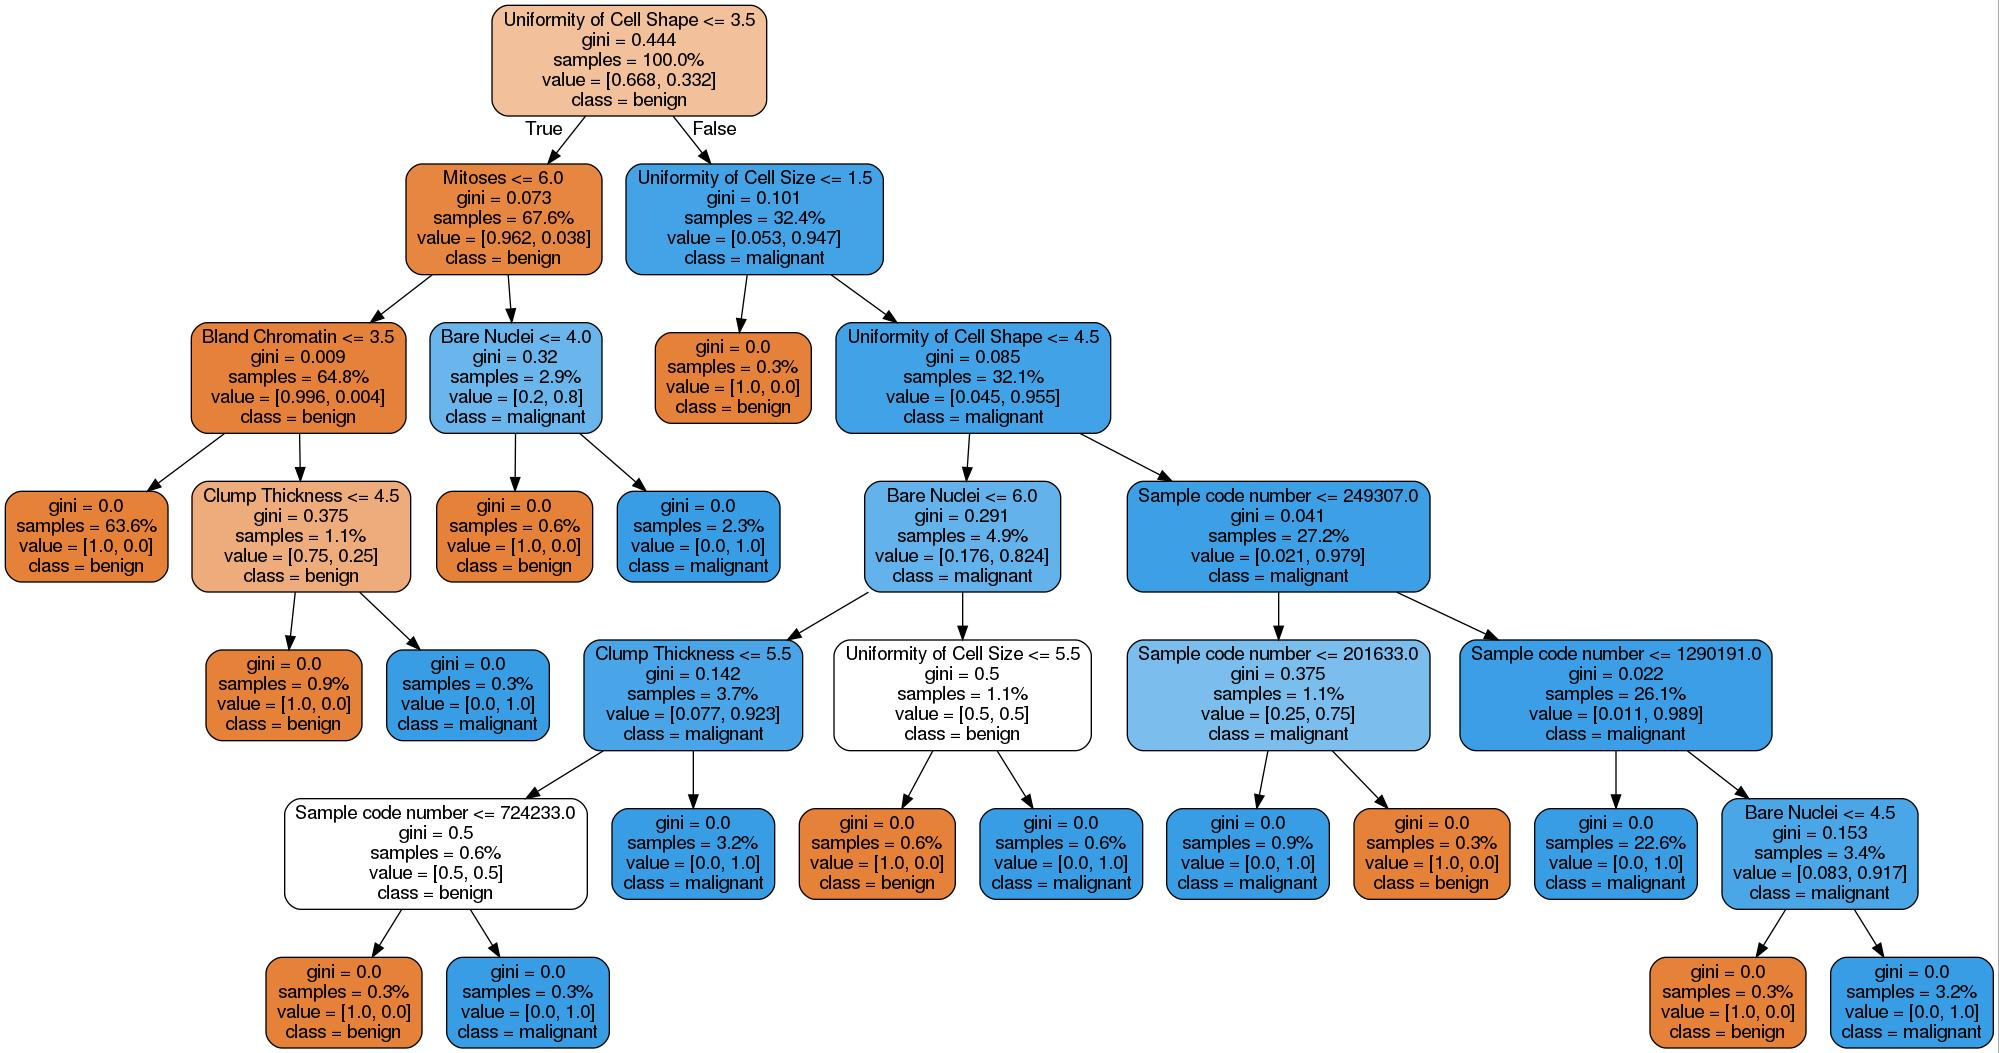
\includegraphics{dtree.jpg}
\caption{Decision tree representation}
\end{figure}

    \subsection{Classification: Regression
Tree}\label{classification-regression-tree}

    \begin{Verbatim}[commandchars=\\\{\}]
{\color{incolor}In [{\color{incolor}50}]:} \PY{k+kn}{from} \PY{n+nn}{sklearn.linear\PYZus{}model} \PY{k+kn}{import} \PY{n}{LogisticRegression}
         \PY{n}{regressionTree} \PY{o}{=} \PY{n}{LogisticRegression}\PY{p}{(}\PY{p}{)}\PY{o}{.}\PY{n}{fit}\PY{p}{(}\PY{n}{X}\PY{o}{=}\PY{n}{xtrain}\PY{p}{,}\PY{n}{y}\PY{o}{=}\PY{n}{ytrain}\PY{p}{)}
         \PY{n}{regressionTreePredicted} \PY{o}{=} \PY{n}{regressionTree}\PY{o}{.}\PY{n}{predict}\PY{p}{(}\PY{n}{xtest}\PY{p}{)}
         \PY{k}{print}\PY{p}{(}\PY{l+s+s2}{\PYZdq{}}\PY{l+s+s2}{Score: }\PY{l+s+si}{\PYZpc{}f}\PY{l+s+s2}{\PYZdq{}} \PY{o}{\PYZpc{}} \PY{n}{regressionTree}\PY{o}{.}\PY{n}{score}\PY{p}{(}\PY{n}{xtest}\PY{p}{,} \PY{n}{ytest}\PY{p}{)}\PY{p}{)}
\end{Verbatim}


    \begin{Verbatim}[commandchars=\\\{\}]
Score: 0.641834

    \end{Verbatim}

    \begin{Verbatim}[commandchars=\\\{\}]
{\color{incolor}In [{\color{incolor}51}]:} \PY{n}{confusion\PYZus{}matrix}\PY{p}{(}\PY{n}{ytrain}\PY{p}{,} \PY{n}{regressionTreePredicted}\PY{p}{)}
\end{Verbatim}


\begin{Verbatim}[commandchars=\\\{\}]
{\color{outcolor}Out[{\color{outcolor}51}]:} array([[233,   0],
                [116,   0]])
\end{Verbatim}
            
    \begin{Verbatim}[commandchars=\\\{\}]
{\color{incolor}In [{\color{incolor}52}]:} \PY{n}{regression\PYZus{}prf} \PY{o}{=} \PY{n}{prf}\PY{p}{(}\PY{n}{ytest}\PY{p}{,} \PY{n}{regressionTreePredicted}\PY{p}{,} \PY{n}{zipResult}\PY{o}{=}\PY{n+nb+bp}{False}\PY{p}{)}
         \PY{n}{regression\PYZus{}prf}
\end{Verbatim}


\begin{Verbatim}[commandchars=\\\{\}]
{\color{outcolor}Out[{\color{outcolor}52}]:} [0.3209169054441261, 0.5, 0.3909249563699826]
\end{Verbatim}
            
    \begin{Verbatim}[commandchars=\\\{\}]
{\color{incolor}In [{\color{incolor}54}]:} \PY{c+c1}{\PYZsh{}\PYZsh{} regression\PYZus{}tree\PYZus{}dot = get\PYZus{}dot\PYZus{}tree(regressionTree, \PYZdq{}regression\PYZus{}tree\PYZus{}dotFile.dot\PYZdq{})}
\end{Verbatim}


    \subsection{Clustering: Kneighbors}\label{clustering-kneighbors}

    \begin{Verbatim}[commandchars=\\\{\}]
{\color{incolor}In [{\color{incolor}20}]:} \PY{k+kn}{from} \PY{n+nn}{sklearn.neighbors} \PY{k+kn}{import} \PY{n}{KNeighborsClassifier} 
         \PY{n}{Nn} \PY{o}{=} \PY{n+nb}{range}\PY{p}{(}\PY{l+m+mi}{1}\PY{p}{,}\PY{l+m+mi}{10}\PY{p}{)}
         
         \PY{k}{def} \PY{n+nf}{forN\PYZus{}kn}\PY{p}{(}\PY{n}{xtrain}\PY{p}{,} \PY{n}{xtest}\PY{p}{,} \PY{n}{ytrain}\PY{p}{,} \PY{n}{ytest}\PY{p}{,} \PY{n}{N}\PY{o}{=}\PY{n}{Nn}\PY{p}{)}\PY{p}{:}
             \PY{n}{resultSet} \PY{o}{=} \PY{p}{[}\PY{p}{]}
             \PY{k}{for} \PY{n}{n} \PY{o+ow}{in} \PY{n}{N}\PY{p}{:}
                 \PY{n}{predicted} \PY{o}{=} \PY{n}{KNeighborsClassifier}\PY{p}{(}\PY{n}{n\PYZus{}neighbors}\PY{o}{=}\PY{n}{n}\PY{p}{)}\PY{o}{.}\PY{n}{fit}\PY{p}{(}\PY{n}{xtrain}\PY{p}{,} \PY{n}{ytrain}\PY{p}{)}\PY{o}{.}\PY{n}{predict}\PY{p}{(}\PY{n}{xtest}\PY{p}{)}
                 \PY{n}{resultSet}\PY{o}{.}\PY{n}{append}\PY{p}{(}\PY{n}{prf}\PY{p}{(}\PY{n}{ytest}\PY{p}{,} \PY{n}{predicted}\PY{p}{,} \PY{n}{zipResult}\PY{o}{=}\PY{n+nb+bp}{False}\PY{p}{)}\PY{p}{)}
             \PY{k}{return} \PY{n}{resultSet}
\end{Verbatim}


    \begin{Verbatim}[commandchars=\\\{\}]
{\color{incolor}In [{\color{incolor}21}]:} \PY{n}{kn\PYZus{}results} \PY{o}{=} \PY{n}{forN\PYZus{}kn}\PY{p}{(}\PY{n}{xtrain}\PY{p}{,} \PY{n}{xtest}\PY{p}{,} \PY{n}{ytrain}\PY{p}{,} \PY{n}{ytest}\PY{p}{)}
         \PY{n}{kn\PYZus{}results}
\end{Verbatim}


\begin{Verbatim}[commandchars=\\\{\}]
{\color{outcolor}Out[{\color{outcolor}21}]:} [[0.5431249541419033, 0.5419821428571429, 0.5423054311943202],
          [0.5838983050847457, 0.5477321428571429, 0.530414096726623],
          [0.5655711677383504, 0.5589999999999999, 0.5593310698953393],
          [0.5795819935691318, 0.5335892857142857, 0.499741987271372],
          [0.5554408807028687, 0.5374107142857143, 0.5258152173913043],
          [0.5875132998936008, 0.541125, 0.5139712488769093],
          [0.558141447368421, 0.537875, 0.5247554599224541],
          [0.6007751937984496, 0.5473571428571429, 0.5218104222821204],
          [0.5868421052631578, 0.5565714285714285, 0.5465223854221889]]
\end{Verbatim}
            
    \begin{Verbatim}[commandchars=\\\{\}]
{\color{incolor}In [{\color{incolor}22}]:} \PY{n}{clustering\PYZus{}prf} \PY{o}{=} \PY{n}{pandas}\PY{o}{.}\PY{n}{DataFrame}\PY{p}{(}\PY{p}{\PYZob{}}
             \PY{l+s+s1}{\PYZsq{}}\PY{l+s+s1}{Index}\PY{l+s+s1}{\PYZsq{}}\PY{p}{:} \PY{p}{[}\PY{l+s+s2}{\PYZdq{}}\PY{l+s+s2}{Clustering N=}\PY{l+s+si}{\PYZpc{}d}\PY{l+s+s2}{\PYZdq{}} \PY{o}{\PYZpc{}} \PY{p}{(}\PY{n}{i}\PY{p}{)} \PY{k}{for} \PY{n}{i} \PY{o+ow}{in} \PY{n}{Nn}\PY{p}{]}\PY{p}{,}
             \PY{l+s+s1}{\PYZsq{}}\PY{l+s+s1}{Precision}\PY{l+s+s1}{\PYZsq{}}\PY{p}{:} \PY{p}{[}\PY{n}{line}\PY{p}{[}\PY{l+m+mi}{0}\PY{p}{]} \PY{k}{for} \PY{n}{line} \PY{o+ow}{in} \PY{n}{kn\PYZus{}results}\PY{p}{]}\PY{p}{,}
             \PY{l+s+s1}{\PYZsq{}}\PY{l+s+s1}{Recal}\PY{l+s+s1}{\PYZsq{}}\PY{p}{:} \PY{p}{[}\PY{n}{line}\PY{p}{[}\PY{l+m+mi}{1}\PY{p}{]} \PY{k}{for} \PY{n}{line} \PY{o+ow}{in} \PY{n}{kn\PYZus{}results}\PY{p}{]}\PY{p}{,}
             \PY{l+s+s1}{\PYZsq{}}\PY{l+s+s1}{F1}\PY{l+s+s1}{\PYZsq{}}\PY{p}{:} \PY{p}{[}\PY{n}{line}\PY{p}{[}\PY{l+m+mi}{2}\PY{p}{]} \PY{k}{for} \PY{n}{line} \PY{o+ow}{in} \PY{n}{kn\PYZus{}results}\PY{p}{]}
         \PY{p}{\PYZcb{}}\PY{p}{)}
\end{Verbatim}


    \begin{Verbatim}[commandchars=\\\{\}]
{\color{incolor}In [{\color{incolor}23}]:} \PY{n}{merged\PYZus{}resultSet} \PY{o}{=} \PY{n}{clustering\PYZus{}prf}\PY{o}{.}\PY{n}{set\PYZus{}index}\PY{p}{(}\PY{l+s+s1}{\PYZsq{}}\PY{l+s+s1}{Index}\PY{l+s+s1}{\PYZsq{}}\PY{p}{)}
         \PY{n}{merged\PYZus{}resultSet}
\end{Verbatim}


\begin{Verbatim}[commandchars=\\\{\}]
{\color{outcolor}Out[{\color{outcolor}23}]:}                       F1  Precision     Recal
         Index                                        
         Clustering N=1  0.542305   0.543125  0.541982
         Clustering N=2  0.530414   0.583898  0.547732
         Clustering N=3  0.559331   0.565571  0.559000
         Clustering N=4  0.499742   0.579582  0.533589
         Clustering N=5  0.525815   0.555441  0.537411
         Clustering N=6  0.513971   0.587513  0.541125
         Clustering N=7  0.524755   0.558141  0.537875
         Clustering N=8  0.521810   0.600775  0.547357
         Clustering N=9  0.546522   0.586842  0.556571
\end{Verbatim}
            
    \subsection{Gather all resultSets}\label{gather-all-resultsets}

    \begin{Verbatim}[commandchars=\\\{\}]
{\color{incolor}In [{\color{incolor}24}]:} \PY{k}{def} \PY{n+nf}{new\PYZus{}pd\PYZus{}single\PYZus{}row}\PY{p}{(}\PY{n}{index\PYZus{}name}\PY{p}{,} \PY{n}{prf}\PY{p}{)}\PY{p}{:}
             \PY{k}{return}  \PY{n}{pandas}\PY{o}{.}\PY{n}{DataFrame}\PY{p}{(}\PY{p}{\PYZob{}}
                 \PY{l+s+s1}{\PYZsq{}}\PY{l+s+s1}{Index}\PY{l+s+s1}{\PYZsq{}}\PY{p}{:} \PY{p}{[}\PY{n}{index\PYZus{}name}\PY{p}{]}\PY{p}{,} 
                 \PY{l+s+s2}{\PYZdq{}}\PY{l+s+s2}{F1}\PY{l+s+s2}{\PYZdq{}}\PY{p}{:} \PY{p}{[}\PY{n}{prf}\PY{p}{[}\PY{l+m+mi}{2}\PY{p}{]}\PY{p}{]}\PY{p}{,} 
                 \PY{l+s+s2}{\PYZdq{}}\PY{l+s+s2}{Recal}\PY{l+s+s2}{\PYZdq{}}\PY{p}{:} \PY{p}{[}\PY{n}{prf}\PY{p}{[}\PY{l+m+mi}{1}\PY{p}{]}\PY{p}{]}\PY{p}{,} 
                 \PY{l+s+s2}{\PYZdq{}}\PY{l+s+s2}{Precision}\PY{l+s+s2}{\PYZdq{}}\PY{p}{:} \PY{p}{[}\PY{n}{prf}\PY{p}{[}\PY{l+m+mi}{0}\PY{p}{]}\PY{p}{]}
             \PY{p}{\PYZcb{}}\PY{p}{)}\PY{o}{.}\PY{n}{set\PYZus{}index}\PY{p}{(}\PY{l+s+s1}{\PYZsq{}}\PY{l+s+s1}{Index}\PY{l+s+s1}{\PYZsq{}}\PY{p}{)}
\end{Verbatim}


    \begin{Verbatim}[commandchars=\\\{\}]
{\color{incolor}In [{\color{incolor}25}]:} \PY{n}{merged\PYZus{}resultSet} \PY{o}{=} \PY{n}{merged\PYZus{}resultSet}\PY{o}{.}\PY{n}{append}\PY{p}{(}\PY{n}{new\PYZus{}pd\PYZus{}single\PYZus{}row}\PY{p}{(}\PY{l+s+s1}{\PYZsq{}}\PY{l+s+s1}{Decision Tree}\PY{l+s+s1}{\PYZsq{}}\PY{p}{,} \PY{n}{decision\PYZus{}prf}\PY{p}{)}\PY{p}{)}
         \PY{n}{merged\PYZus{}resultSet} \PY{o}{=} \PY{n}{merged\PYZus{}resultSet}\PY{o}{.}\PY{n}{append}\PY{p}{(}\PY{n}{new\PYZus{}pd\PYZus{}single\PYZus{}row}\PY{p}{(}\PY{l+s+s1}{\PYZsq{}}\PY{l+s+s1}{Regression Tree}\PY{l+s+s1}{\PYZsq{}}\PY{p}{,} \PY{n}{regression\PYZus{}prf}\PY{p}{)}\PY{p}{)}
         \PY{n}{merged\PYZus{}resultSet}
\end{Verbatim}


\begin{Verbatim}[commandchars=\\\{\}]
{\color{outcolor}Out[{\color{outcolor}25}]:}                        F1  Precision     Recal
         Index                                         
         Clustering N=1   0.542305   0.543125  0.541982
         Clustering N=2   0.530414   0.583898  0.547732
         Clustering N=3   0.559331   0.565571  0.559000
         Clustering N=4   0.499742   0.579582  0.533589
         Clustering N=5   0.525815   0.555441  0.537411
         Clustering N=6   0.513971   0.587513  0.541125
         Clustering N=7   0.524755   0.558141  0.537875
         Clustering N=8   0.521810   0.600775  0.547357
         Clustering N=9   0.546522   0.586842  0.556571
         Decision Tree    0.937679   0.937679  0.937679
         Regression Tree  0.390925   0.320917  0.500000
\end{Verbatim}
            

    % Add a bibliography block to the postdoc
    
    
    
    \end{document}
